%=======================================================================
%  CHAPTER 7 — APPLICATIONS OF AI : SOLVED PROBLEMS
%=======================================================================
\section{Applications of AI \textcolor{sub}{\large -- Solved Problems}}

{\color{sub}\footnotesize Every problem opens with the question
\mk{exactly as the paper prints it}, the paper's own spelling and slips
included. \gap$\cdot$\gap \textbf{The gate networks} (17 papers), \textbf{the Hebbian
AND net} (4), \textbf{the Hopfield weight matrix} (1 at 6 marks), \textbf{the printed
forward-propagation network} (2 at 8 marks each) and \textbf{the parse tree} (1).
\gap$\cdot$\gap Every weight, net input, activation and matrix entry printed here is
recomputed independently by \code{verify.py}.}

\lead{\mk{Three things to know before you start.}}
\begin{itemize}
  \item \mk{Use bipolar values, $\pm 1$, not 0 and 1.} With binary
        inputs a 0 contributes nothing to any weight update, so the Hebb net for AND
        \emph{cannot be learnt at all} and the perceptron takes six epochs instead of
        two. Every worked answer below uses $\pm 1$ and says so in its first line.
  \item \mk{``Design'' and ``train'' are different questions.}
        \emph{Design} a net for AND: choose weights, verify the four rows, done in five
        lines. \emph{Construct it using the perceptron / Hebb algorithm and show each
        calculation}: run the table. Read which one the paper asked $-$
        \yr{\textbf{\textit{77 Ch}}} says \emph{``show each calculation performed''} and
        will not accept a designed answer.
  \item \mk{Always finish with the verification table.} Four rows,
        $net$ and $y$ against the target. It is two minutes, it catches every arithmetic
        slip, and the marks for it are free.
\end{itemize}

\hr

%=======================================================================
\T{7.N.1 Problem 1.1 --- McCulloch-Pitts neuron for AND and OR}

\creamq{What is a McCulloch/Pitts neural network? Explain it with reference to the AND gate}{\m{8}\m{10}}
{\color{sub}\footnotesize \tP{2} \yr{75 Ba \m{8}, 76 Ba \m{10}} \gap$\cdot$\gap
both papers then ask \emph{why it cannot do XOR}, which is Problem 1.4
\gap$\cdot$\gap \mk{the MP neuron's weights are chosen, not learnt},
so this problem is solved by \textbf{inequalities}, never by a training table}

\begin{asked}{75 Ba \textperiodcentered{} Q9 \textperiodcentered{} \m{8}}
What is a McCulloch/Pitts neural network? Explain it with reference to AND gate. Justify
that it cannot be applied to Exclusive OR gate.
\end{asked}

\sbsr{0.50}{%
\lead{Step 1 \gap Write the network and the firing condition}
\begin{itemize}
  \item Two inputs $x_1, x_2$, weights $w_1, w_2$, threshold $T$. The neuron fires
        ($y=1$) exactly when
        \[ x_1 w_1 + x_2 w_2 > T \]
  \item \mk{Nothing is learnt.} The task is to find one $(w_1, w_2, T)$
        that makes the four rows come out right.
\end{itemize}
\lead{Step 2 \gap One inequality per row of the truth table}
\begin{tabularx}{\linewidth}{@{}ccXX@{}}
\hrow \thead{$x_1$} & \thead{$x_2$} & \thead{AND target} & \thead{Condition} \\
0 & 0 & 0 & $0 \le T$ \hfill (i) \\
0 & 1 & 0 & $w_2 \le T$ \hfill (ii) \\
1 & 0 & 0 & $w_1 \le T$ \hfill (iii) \\
1 & 1 & 1 & $w_1 + w_2 > T$ \hfill (iv) \\
\end{tabularx}
\lead{Step 3 \gap Solve them}
\begin{itemize}
  \item (ii) and (iii) say each weight alone must \emph{not} reach the threshold;
        (iv) says the two together must pass it. So pick $w_1 = w_2 = w$ and
        \mk{any $T$ with $w \le T < 2w$}.
  \item Take $w_1 = w_2 = 1$ and $T = 1.5$. Or, as the deck does, $w_1 = w_2 = 0.7$ and
        $T = 1$.
\end{itemize}}{%
\lead{Step 4 \gap Verify all four rows}
\begin{tabularx}{\linewidth}{@{}ccXXX@{}}
\hrow \thead{$x_1$} & \thead{$x_2$} & \thead{$net = x_1 + x_2$} &
  \thead{$net > 1.5$?} & \thead{$y$} \\
0 & 0 & 0 & no  & 0 \checkmark \\
0 & 1 & 1 & no  & 0 \checkmark \\
1 & 0 & 1 & no  & 0 \checkmark \\
1 & 1 & 2 & yes & \mk{1} \checkmark \\
\end{tabularx}
\par\penalty0\vspace{2pt}
\noindent\colorbox{gdL}{\parbox{\dimexpr\linewidth-2\fboxsep}{\textbf{AND.}
$w_1 = w_2 = \mathbf{1}$, $T = \mathbf{1.5}$.}}
\lead{The OR gate, same method}
\begin{itemize}
  \item Rows: $0 \le T$; $w_2 > T$; $w_1 > T$; $w_1 + w_2 > T$. Now \emph{either} weight
        alone must pass, so \mk{$0 \le T < w$}.
  \item Take $w_1 = w_2 = 1$, $T = 0.5$: $net = 0$ (no), $1$ (yes), $1$ (yes),
        $2$ (yes). \checkmark
\end{itemize}
\lead{NOT, for completeness}
\begin{itemize}
  \item One \textbf{inhibitory} input: $w = -1$, $T = -0.5$.
        $x=0 \rightarrow net = 0 > -0.5 \rightarrow y=1$;
        $x=1 \rightarrow net = -1 \rightarrow y=0$. \checkmark
  \item \mk{AND, OR and NOT together make every Boolean function}, so
        a \emph{network} of MP neurons is universal even though one neuron is not. That
        sentence is what \yr{76 Ba}'s \emph{``propose a neural network model''} wants.
\end{itemize}}

%=======================================================================
\T{7.N.2 Problem 1.2 --- train a perceptron to be an AND gate}

\creamq{Write down the perceptron algorithm and use it to construct a network which performs like a logical AND operation, showing each calculation}{\m{2+6}\m{2+2+4}}
{\color{sub}\footnotesize \tF{4} \yr{\textbf{\textit{77 Ch}} \m{2+6},
\textbf{\textit{73 Bh}} \m{2+6}, 78 Po \m{2+2+4}, 79 Jth \m{1+6}} \gap$\cdot$\gap
\yr{\textbf{\textit{77 Ch}}} says \mk{``show each calculation
performed''}, so the table below is the answer and a designed set of weights is
not \gap$\cdot$\gap \yr{79 Jth} says \emph{``acts as logic gates''}, so give AND and add
OR from Problem 1.3}

\begin{asked}{\textbf{\textit{77 Ch}} \textperiodcentered{} Q9 \textperiodcentered{} \m{2+6}}
Why do you need Multilayer Perceptron Neural Networks? Write down the perceptron
algorithm and use it to Construct Network which perform like Logical AND Operation and
show each calculation performed.
\end{asked}

\sbsr{0.44}{%
\lead{Step 1 \gap Set up}
\begin{itemize}
  \item \textbf{Bipolar} inputs and targets, $\pm 1$. Bias input fixed at $+1$.
  \item Learning rate $\alpha = 1$, threshold $\theta = 0$.
  \item Start with $w_1 = w_2 = b = 0$.
  \item \textbf{Activation}: $y = 1$ if $net > 0$, $y = 0$ if $net = 0$, $y = -1$ if
        $net < 0$.
  \item \textbf{Update, only when $y \neq t$:}
        \[ w_i \leftarrow w_i + \alpha\,t\,x_i, \qquad b \leftarrow b + \alpha\,t \]
  \item \mk{$net = 0$ counts as an error}, because $y=0$ never equals
        a target of $\pm 1$. That is what makes the very first row update.
\end{itemize}
\lead{Truth table, in bipolar form}
\begin{tabularx}{\linewidth}{@{}XXXX@{}}
\hrow \thead{$x_1$} & \thead{$x_2$} & \thead{AND} & \thead{$t$} \\
1 & 1 & 1 & $+1$ \\
1 & $-1$ & 0 & $-1$ \\
$-1$ & 1 & 0 & $-1$ \\
$-1$ & $-1$ & 0 & $-1$ \\
\end{tabularx}}{%
\lead{Step 2 \gap Epoch 1}
\begin{tabularx}{\linewidth}{@{}L{1.5cm}L{1.5cm}ccL{2.4cm}XXX@{}}
\hrow \thead{$(x_1,x_2)$} & \thead{$net$} & \thead{$y$} & \thead{$t$} &
  \thead{Update} & \thead{$w_1$} & \thead{$w_2$} & \thead{$b$} \\
start & & & & & 0 & 0 & 0 \\
$(1,1)$ & $0$ & 0 & $+1$ & $y \neq t$, add $t\,x_i$ & 1 & 1 & 1 \\
$(1,-1)$ & $1$ & 1 & $-1$ & $y \neq t$ & 0 & 2 & 0 \\
$(-1,1)$ & $2$ & 1 & $-1$ & $y \neq t$ & 1 & 1 & $-1$ \\
$(-1,-1)$ & $-3$ & $-1$ & $-1$ & \mk{correct, no change} & 1 & 1 & $-1$ \\
\end{tabularx}
{\color{sub}\footnotesize Sample working, row 2: $net = b + w_1x_1 + w_2x_2
= 1 + 1(1) + 1(-1) = 1$, so $y=1$ but $t=-1$. Then
$w_1 = 1 + (-1)(1) = 0$, $w_2 = 1 + (-1)(-1) = 2$, $b = 1 + (-1) = 0$.}
\lead{Step 3 \gap Epoch 2 --- the verification pass}
\begin{tabularx}{\linewidth}{@{}L{1.6cm}L{2.6cm}XXX@{}}
\hrow \thead{$(x_1,x_2)$} & \thead{$net = -1 + x_1 + x_2$} & \thead{$y$} &
  \thead{$t$} & \thead{} \\
$(1,1)$ & $-1+1+1 = 1$ & $1$ & $+1$ & \checkmark \\
$(1,-1)$ & $-1+1-1 = -1$ & $-1$ & $-1$ & \checkmark \\
$(-1,1)$ & $-1-1+1 = -1$ & $-1$ & $-1$ & \checkmark \\
$(-1,-1)$ & $-1-1-1 = -3$ & $-1$ & $-1$ & \checkmark \\
\end{tabularx}
\par\penalty0\vspace{2pt}
\noindent\colorbox{gdL}{\parbox{\dimexpr\linewidth-2\fboxsep}{\textbf{Answer.}
No weight changed in epoch 2, so the perceptron has \textbf{converged after one epoch of
updates}: $\mathbf{w_1 = 1}$, $\mathbf{w_2 = 1}$, $\mathbf{b = -1}$.
Decision line $x_1 + x_2 = 1$.}}}

%=======================================================================
\T{7.N.3 Problem 1.3 --- train a perceptron to be an OR gate}

\creamq{How can we design a neural network that acts as an OR gate?}{\m{2+7}}
{\color{sub}\footnotesize \yr{72 Ma} \m{2+7} \gap$\cdot$\gap
\mk{OR converges even faster than AND} $-$ one row of updates and it
is done \gap$\cdot$\gap only the target column changes from Problem 1.2, so if you have
written that one, say so and change the column}

\begin{asked}{72 Ma \textperiodcentered{} Q8 \textperiodcentered{} \m{2+7}}
What do you understand by a perceptron? How can we design a neural network that acts as
an OR gate.
\end{asked}

\sbs{%
\lead{Same setup, one column different}
\begin{tabularx}{\linewidth}{@{}L{1.5cm}L{1.4cm}ccXXX@{}}
\hrow \thead{$(x_1,x_2)$} & \thead{$net$} & \thead{$y$} & \thead{$t$} &
  \thead{$w_1$} & \thead{$w_2$} & \thead{$b$} \\
start & & & & 0 & 0 & 0 \\
$(1,1)$ & $0$ & 0 & $+1$ & 1 & 1 & 1 \\
$(1,-1)$ & $1$ & 1 & $+1$ & 1 & 1 & 1 \\
$(-1,1)$ & $1$ & 1 & $+1$ & 1 & 1 & 1 \\
$(-1,-1)$ & $-1$ & $-1$ & $-1$ & 1 & 1 & 1 \\
\end{tabularx}
\begin{itemize}
  \item \mk{Only the first row ever updates.} After it, every
        remaining pattern is already classified correctly, so the weights are untouched.
  \item Epoch 2 confirms: $net = 3, 1, 1, -1$ against targets $+1,+1,+1,-1$. \checkmark
\end{itemize}
\par\penalty0\vspace{2pt}
\noindent\colorbox{gdL}{\parbox{\dimexpr\linewidth-2\fboxsep}{\textbf{Answer.}
$\mathbf{w_1 = 1}$, $\mathbf{w_2 = 1}$, $\mathbf{b = +1}$. Decision line
$x_1 + x_2 = -1$.}}}{%
\lead{AND and OR side by side, which is worth a sentence}
\begin{tabularx}{\linewidth}{@{}L{2.4cm}XX@{}}
\hrow \thead{} & \thead{AND} & \thead{OR} \\
$w_1, w_2$ & 1, 1 & 1, 1 \\
Bias $b$ & \mk{$-1$} & \mk{$+1$} \\
Fires when & both inputs are $+1$ & at least one is $+1$ \\
Epochs of updates & 1 (three updates) & 1 (one update) \\
\end{tabularx}
\begin{itemize}
  \item \mk{The weights are identical; only the bias moves.} The bias
        slides the same decision line across the square: with $b=-1$ it cuts off the
        single corner $(1,1)$, with $b=+1$ it cuts off the single corner $(-1,-1)$.
  \item That is the cleanest statement of what a bias \emph{is} for, and it is the answer
        to \yr{79 Jth}'s \emph{``can we design a neural network that acts as logic
        gates''}: yes, and the same network does both, with one number changed.
  \item \textbf{NAND} is AND with the targets flipped, giving $w_1=w_2=-1$, $b=+1$; and
        \textbf{NOR} is OR flipped. Both are needed in Problem 1.4.
\end{itemize}}

%=======================================================================
\T{7.N.4 Problem 1.4 --- XOR: the proof, and the network that does work}

\creamq{Is a single perceptron sufficient to realize a network behaving as an XOR gate? Justify. How can we design one that does?}{\m{6}\m{10}\m{1+8}\m{2+6}\m{1+7}}
{\color{sub}\footnotesize \tS{8} \yr{73 Ma \m{1+7}, \textit{74 Ma} \m{10},
\textbf{\textit{74 Bh}} \m{1+8}, \textbf{\texttt{82 Bh}} \m{2+6}, 79 Ash \m{1+8},
\textbf{77 Ch} \m{2+6}, 76 Ba \m{10}, 75 Ba \m{8}} \gap$\cdot$\gap
\mk{eight papers, and the answer has two halves}: prove one neuron
cannot, then build one that can. Doing only the first half costs half the marks, and
doing only the second costs more}

\begin{asked}{79 Ash \textperiodcentered{} Q8 \textperiodcentered{} \m{1+8}}
What is perceptron? Is single perceptron sufficient to realize a network behaving as XOR
gate? Justify.
\end{asked}

\sbsr{0.50}{%
\lead{Part 1 \gap Why one perceptron cannot: the geometric answer}
\begin{itemize}
  \item Plot the four inputs on the unit square. XOR outputs 1 at $(0,1)$ and $(1,0)$,
        and 0 at $(0,0)$ and $(1,1)$.
  \item The two 1s are at \mk{diagonally opposite} corners, and so are
        the two 0s. \textbf{No straight line puts one pair on one side and the other pair
        on the other.}
  \item A single neuron computes $w_1x_1 + w_2x_2 + b$ and thresholds it, and the
        boundary of a threshold is exactly a straight line. So it cannot be done.
        \mk{Draw the square with the two attempted lines.}
\end{itemize}
\lead{Part 1 again \gap The algebraic proof, if the paper says ``justify''}
\begin{itemize}
  \item Assume $w_1, w_2, b$ exist with output 1 iff $w_1x_1 + w_2x_2 + b > 0$:
  \begin{itemize}
    \item $(0,0) \rightarrow 0$: \quad $b \le 0$ \hfill (i)
    \item $(0,1) \rightarrow 1$: \quad $w_2 + b > 0$ \hfill (ii)
    \item $(1,0) \rightarrow 1$: \quad $w_1 + b > 0$ \hfill (iii)
    \item $(1,1) \rightarrow 0$: \quad $w_1 + w_2 + b \le 0$ \hfill (iv)
  \end{itemize}
  \item Adding (ii) and (iii): $w_1 + w_2 + 2b > 0$, so $w_1 + w_2 > -2b$.
  \item But (iv) gives $w_1 + w_2 \le -b$. Hence $-2b < -b$, i.e.
        \mk{$b > 0$}, contradicting (i).
  \item \textbf{No such weights exist.} $\blacksquare$
  \item \mk{Say what this does not mean}: it is a limit on \emph{one}
        neuron, not on neural networks. XOR is not a hard function; it is a
        \emph{non-linearly-separable} one.
\end{itemize}}{%
\lead{Part 2 \gap The two-layer network that does work}
\begin{itemize}
  \item \textbf{The idea in one line}:
        $x_1 \oplus x_2 \;=\; (x_1 \lor x_2) \;\land\; \lnot(x_1 \land x_2)$.
        So build OR and AND in a hidden layer and combine them at the output.
  \item \textbf{The network} (binary inputs, step activation, fire if $net > 0$):
  \begin{itemize}
    \item Hidden $h_1$ $=$ \textbf{OR}: \quad $w = (1,\,1)$, $b = -0.5$
    \item Hidden $h_2$ $=$ \textbf{AND}: \quad $w = (1,\,1)$, $b = -1.5$
    \item Output $y$: \quad $w = (+1 \text{ from } h_1,\; -1 \text{ from } h_2)$,
          $b = -0.5$
  \end{itemize}
\end{itemize}
\lead{Verification, all four rows}
\begin{tabularx}{\linewidth}{@{}ccXXXXX@{}}
\hrow \thead{$x_1$} & \thead{$x_2$} & \thead{$net_1$} & \thead{$h_1$} &
  \thead{$net_2$} & \thead{$h_2$} & \thead{$y$} \\
0 & 0 & $-0.5$ & 0 & $-1.5$ & 0 & $-0.5 \rightarrow \mathbf{0}$ \\
0 & 1 & $0.5$  & 1 & $-0.5$ & 0 & $0.5 \rightarrow \mathbf{1}$ \\
1 & 0 & $0.5$  & 1 & $-0.5$ & 0 & $0.5 \rightarrow \mathbf{1}$ \\
1 & 1 & $1.5$  & 1 & $0.5$  & 1 & $-0.5 \rightarrow \mathbf{0}$ \\
\end{tabularx}
\par\penalty0\vspace{2pt}
\noindent\colorbox{gdL}{\parbox{\dimexpr\linewidth-2\fboxsep}{\textbf{Answer.} A single
perceptron cannot. A \textbf{2--2--1 multilayer perceptron} can: hidden units computing
OR and AND, output computing $h_1 - h_2 - 0.5$. Output column matches XOR exactly.}}
\begin{itemize}
  \item \mk{Why it works, geometrically}: each hidden unit draws one
        straight line, and the output unit takes the strip \emph{between} them. Two lines
        can isolate a diagonal pair; one cannot.
  \item \mk{And why it needs back-propagation to be \emph{learnt}}:
        the hidden units have no targets of their own, so no perceptron rule can train
        them. This is the answer to \yr{\textbf{\textit{77 Ch}}}'s \emph{``why do you
        need multilayer perceptron networks''} and to \yr{\textbf{79 Ch}}'s
        \emph{``when do we need the back propagation algorithm''}. One step of it is
        Problem 2.2.
\end{itemize}}

%=======================================================================
\T{7.N.5 Problem 1.5 --- a Hebbian network for AND}

\creamq{Define Hebbian learning. Use the Hebbian learning algorithm to construct a network which performs the AND function}{\m{2+6}\m{1+7}\m{3+7}\m{6+3}}
{\color{sub}\footnotesize \tF{4} \yr{\textbf{73 Bh} \m{3+7}, \texttt{81 Ba} \m{2+6},
78 Ba \m{1+7}, \textbf{78 Ch} \m{6+3}} \gap$\cdot$\gap
\mk{one pass, no iteration, no error term} $-$ that is what makes it
different from Problem 1.2 and it is what the examiner checks \gap$\cdot$\gap
\yr{\textbf{78 Ch}} also asks \emph{is Hebbian learning supervised? Justify}}

\begin{asked}{\texttt{81 Ba} \textperiodcentered{} Q8 \textperiodcentered{} \m{2+6}}
What is perception? Construct a Hebbian Network that performs like AND Gate.
\end{asked}

\sbsr{0.53}{%
\lead{Step 1 \gap The rule}
\begin{itemize}
  \item Bipolar inputs and targets; bias input fixed at $+1$; all weights start at
        \textbf{0}.
  \item For each training pair, \mk{set the output to the target} and
        update:
        \[ w_i \leftarrow w_i + x_i\,t, \qquad b \leftarrow b + t \]
  \item \mk{No learning rate, no comparison, no second pass.} Every
        pattern updates, whether the current weights would have got it right or not.
\end{itemize}
\lead{Step 2 \gap One pass through the four patterns}
\begin{tabularx}{\linewidth}{@{}L{1.6cm}cL{3.6cm}XXX@{}}
\hrow \thead{$(x_1,x_2)$} & \thead{$t$} & \thead{Working} &
  \thead{$w_1$} & \thead{$w_2$} & \thead{$b$} \\
start & & & 0 & 0 & 0 \\
$(1,1)$ & $+1$ & $0{+}(1)(1)$, $0{+}(1)(1)$, $0{+}1$ & 1 & 1 & 1 \\
$(1,-1)$ & $-1$ & $1{+}(1)(-1)$, $1{+}(-1)(-1)$, $1{-}1$ & 0 & 2 & 0 \\
$(-1,1)$ & $-1$ & $0{+}(-1)(-1)$, $2{+}(1)(-1)$, $0{-}1$ & 1 & 1 & $-1$ \\
$(-1,-1)$ & $-1$ & $1{+}(-1)(-1)$, $1{+}(-1)(-1)$, $-1{-}1$ &
  \mk{2} & \mk{2} & \mk{$-2$} \\
\end{tabularx}}{%
\lead{Step 3 \gap Verify}
\begin{tabularx}{\linewidth}{@{}L{1.6cm}L{3.4cm}XXX@{}}
\hrow \thead{$(x_1,x_2)$} & \thead{$net = 2x_1 + 2x_2 - 2$} & \thead{$y$} &
  \thead{$t$} & \thead{} \\
$(1,1)$   & $2+2-2 = 2$   & $1$  & $+1$ & \checkmark \\
$(1,-1)$  & $2-2-2 = -2$  & $-1$ & $-1$ & \checkmark \\
$(-1,1)$  & $-2+2-2 = -2$ & $-1$ & $-1$ & \checkmark \\
$(-1,-1)$ & $-2-2-2 = -6$ & $-1$ & $-1$ & \checkmark \\
\end{tabularx}
\par\penalty0\vspace{2pt}
\noindent\colorbox{gdL}{\parbox{\dimexpr\linewidth-2\fboxsep}{\textbf{Answer.}
$\mathbf{w_1 = 2}$, $\mathbf{w_2 = 2}$, $\mathbf{b = -2}$, from
\textbf{one pass}. Decision line $x_1 + x_2 = 1$ $-$ the same line the perceptron found
in Problem 1.2, at twice the scale.}}
\lead{Is Hebbian learning supervised? \gap{\color{sub}\footnotesize(\yr{\textbf{78 Ch}} \m{3})}}
\begin{itemize}
  \item \mk{Yes, as used here.} The update contains $t$, the target,
        so the network is being told the right answer for every pattern. Without $t$
        there is no AND net.
  \item \mk{But Hebb's original postulate is not.} \emph{Neurons that
        fire together wire together} describes a purely local, unsupervised change in a
        synapse; nothing in it mentions a desired output.
  \item So the honest answer is both sentences: the \emph{principle} is unsupervised,
        the \emph{Hebb net for pattern association} is supervised because it substitutes
        the target for the output.
  \item \mk{Why bipolar is compulsory here.} With binary values, the
        pattern $(0,0)$ contributes $0 \times t = 0$ to both weights, so it can never
        push the weights away from a wrong answer. Run the same table in binary and the
        AND net comes out wrong. Say this if you have room; it is the trap the question
        is built on.
\end{itemize}}

\hr

%=======================================================================
\T{7.N.6 Problem 2.1 --- forward propagation through the printed network}

\creamq{Perform forward propagation, and update the weights of the second hidden layer, a and b}{\m{8}}
{\color{sub}\footnotesize \tP{2} \yr{82 Ka \m{8}, \textbf{81 Ch} \m{8}} \gap$\cdot$\gap
\mk{the same question printed twice, with the same figure}
\gap$\cdot$\gap the paper gives \textbf{no target value and no learning rate}, so both
are assumed below and stated \gap$\cdot$\gap
\mk{the interesting part is what happens to c, d, e and f}}

\begin{asked}{82 Ka \textperiodcentered{} Q7 \textperiodcentered{} \m{8} \gap\textperiodcentered{}\gap identical at \textbf{81 Ch} \textperiodcentered{} Q9}
Below is a neural network with weights a, b, c, d, e, and f. The input are $x_1$ and
$x_2$. The first hidden layer computes $r_1 = \max(c.x_1 + e.x_2,\ 0)$ and
$r_2 = \max(d.x_1 + f.x_2,\ 0)$. The second hidden layer and third layer computes $s_1$,
$s_2$ and $y$ using sigmoid activation function. Suppose the network has inputs
$x_1 = -1$ and $x_2 = -1$. The weight values are a $=$ 1, b $=$ 1, c $=$ 4, d $=$ 1,
e $=$ 2 and f $=$ 2. Perform forward propagation. And update weight for second hidden
layer for a and b.
\par\penalty0\vspace{2pt}
\mbox{}\hfill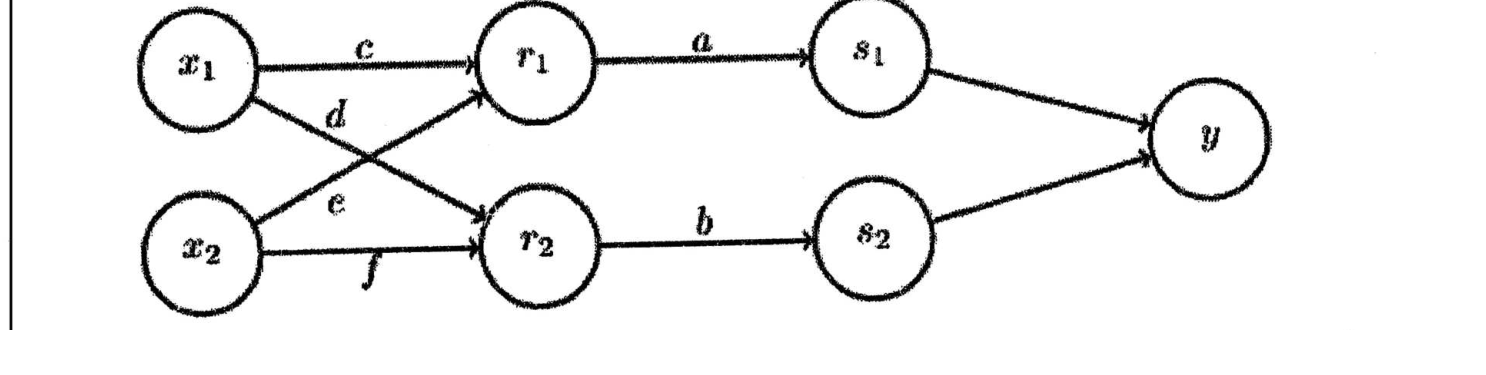
\includegraphics[width=3.9in]{figs/c7_82ka_ann.png}\hfill\mbox{}
\end{asked}

\sbsr{0.50}{%
\lead{Step 1 \gap Read the network off the figure}
\begin{itemize}
  \item $x_1 \rightarrow r_1$ with weight $c$, $x_2 \rightarrow r_1$ with weight $e$;
        $x_1 \rightarrow r_2$ with $d$, $x_2 \rightarrow r_2$ with $f$.
  \item $r_1 \rightarrow s_1$ and $r_2 \rightarrow s_2$ apply the \textbf{sigmoid}.
  \item $s_1 \rightarrow y$ with weight $a$, $s_2 \rightarrow y$ with $b$, then sigmoid
        again. \mk{No biases anywhere}, which the figure confirms.
  \item $\max(z, 0)$ is the \textbf{ReLU}; $\sigma(z) = 1/(1+e^{-z})$.
\end{itemize}
\lead{Step 2 \gap First hidden layer}
\begin{align*}
 r_1 &= \max(c\,x_1 + e\,x_2,\; 0) = \max(4(-1) + 2(-1),\; 0) \\
     &= \max(-6,\; 0) = \mathbf{0} \\
 r_2 &= \max(d\,x_1 + f\,x_2,\; 0) = \max(1(-1) + 2(-1),\; 0) \\
     &= \max(-3,\; 0) = \mathbf{0}
\end{align*}
\lead{Step 3 \gap Second hidden layer and output}
\begin{align*}
 s_1 &= \sigma(r_1) = \sigma(0) = \tfrac{1}{1+e^{0}} = \mathbf{0.5} \\
 s_2 &= \sigma(r_2) = \sigma(0) = \mathbf{0.5} \\
 net_y &= a\,s_1 + b\,s_2 = 1(0.5) + 1(0.5) = 1 \\
 y &= \sigma(1) = \tfrac{1}{1+e^{-1}} = \mathbf{0.7311}
\end{align*}
\par\penalty0\vspace{2pt}
\noindent\colorbox{gdL}{\parbox{\dimexpr\linewidth-2\fboxsep}{\textbf{Forward pass.}
$r_1 = r_2 = 0$, \; $s_1 = s_2 = 0.5$, \; $\mathbf{y = 0.7311}$.}}}{%
\lead{Step 4 \gap Update a and b}
{\color{sub}\footnotesize The paper gives no target and no learning rate. Assume
\mk{$t = 1$} and \mk{$\eta = 0.1$}, and say so $-$
the method is what is marked, and any other pair of values substitutes into the same
three lines.}
\begin{itemize}
  \item Loss $E = \tfrac12 (y-t)^2$. Output delta:
        \[ \delta = (y-t)\,y\,(1-y) \]
        \[ = (0.7311 - 1)(0.7311)(0.2689) = \mathbf{-0.05288} \]
  \item Gradients, since the input to both weights is $0.5$:
        \[ \frac{\partial E}{\partial a} = \delta\,s_1 = -0.05288 \times 0.5
           = -0.02644 \]
        and $\partial E / \partial b$ is the same, because $s_1 = s_2$.
  \item Update:
        \begin{align*}
        a &\leftarrow a - \eta\,\frac{\partial E}{\partial a}
           = 1 - 0.1(-0.02644) = \mathbf{1.00264} \\
        b &\leftarrow b - \eta\,\frac{\partial E}{\partial b} = \mathbf{1.00264}
        \end{align*}
  \item \mk{Both weights rise}, and by the same amount, because the
        output was below the target and both units fed it the same 0.5.
\end{itemize}
\lead{\mk{The part worth extra marks: c, d, e and f cannot be updated at all}}
\begin{itemize}
  \item The gradient reaching $c$ runs through $r_1 = \max(-6, 0)$. The derivative of
        ReLU at a negative input is \textbf{0}, so
        $\partial E/\partial c = \partial E/\partial d = \partial E/\partial e =
         \partial E/\partial f = 0$.
  \item Both hidden units are \mk{dead for this input}: no gradient
        flows past them, so the first layer learns nothing from this example. This is the
        textbook \textbf{dying-ReLU} problem, and it is precisely why the question asks
        you to update only $a$ and $b$.
  \item Saying that explicitly is what turns a correct arithmetic answer into a complete
        one.
\end{itemize}}

%=======================================================================
\T{7.N.7 Problem 2.2 --- one full step of back-propagation}

\creamq{Explain the back-propagation algorithm with an example}{\m{4}\m{2+6}\m{3+5}\m{4+4}}
{\color{sub}\footnotesize \tS{8} \yr{\textbf{70 Bh} \m{4+4},
\textbf{72 Ash} \m{2+4+4}, 70 Ma \m{3+5}, \textbf{\texttt{80 Bh}} \m{2+2+4},
\textbf{74 Bh} \m{4}, \textbf{79 Ch} \m{2+6}, 71 Ma \m{3+5},
\textbf{\textit{72 Ash}} \m{3+5}} \gap$\cdot$\gap
\mk{no paper supplies numbers}, so this is the standard XOR network
with the weights every deck uses \gap$\cdot$\gap one input pattern and one step is
enough for 6 marks; do not attempt a full epoch}

\begin{asked}[PROBLEM]{not a PYQ \textperiodcentered{} the 2--2--1 XOR network, with the weights the lecture decks use}
Train the network below on the XOR pattern $x = (1, 1)$, target $t = 0$, for one step.
Sigmoid activation, loss $E = \tfrac12 (y-t)^2$, learning rate $\eta = 0.1$.
Initial weights $w_{13}=0.5$, $w_{14}=0.9$, $w_{23}=0.4$, $w_{24}=1.0$,
$w_{35}=-1.2$, $w_{45}=1.1$; biases $b_3=-0.8$, $b_4=0.1$, $b_5=-0.3$.
\end{asked}

\sbsr{0.48}{%
\lead{Step 1 \gap Forward pass}
\begin{align*}
 net_3 &= x_1w_{13} + x_2w_{23} + b_3 = 0.5 + 0.4 - 0.8 = 0.1 \\
 h_3 &= \sigma(0.1) = \tfrac{1}{1+e^{-0.1}} = \mathbf{0.5250} \\
 net_4 &= x_1w_{14} + x_2w_{24} + b_4 = 0.9 + 1.0 + 0.1 = 2.0 \\
 h_4 &= \sigma(2.0) = \mathbf{0.8808} \\
 net_5 &= h_3w_{35} + h_4w_{45} + b_5 \\
       &= 0.5250(-1.2) + 0.8808(1.1) - 0.3 = 0.0389 \\
 y_5 &= \sigma(0.0389) = \mathbf{0.5097}
\end{align*}
\begin{itemize}
  \item Error $E = \tfrac12(0.5097 - 0)^2 = \mathbf{0.1299}$.
\end{itemize}
\lead{Step 2 \gap Output delta}
\[ \delta_5 = (y_5 - t)\,y_5(1-y_5) \]
\[ = (0.5097)(0.5097)(0.4903) = \mathbf{0.12738} \]
{\color{sub}\footnotesize $y(1-y)$ is the derivative of the sigmoid, and the forward pass
already gave you $y$ $-$ that is the whole reason sigmoid is used.}
\lead{Step 3 \gap Hidden deltas}
\begin{align*}
 \delta_3 &= \delta_5\,w_{35}\,h_3(1-h_3) \\
          &= 0.12738(-1.2)(0.5250)(0.4750) = \mathbf{-0.03812} \\
 \delta_4 &= \delta_5\,w_{45}\,h_4(1-h_4) \\
          &= 0.12738(1.1)(0.8808)(0.1192) = \mathbf{0.01471}
\end{align*}
\begin{itemize}
  \item \mk{$\delta_3$ is negative because $w_{35}$ is}: unit 3 pushes
        the output \emph{down}, so to reduce an output that is too high you must push
        unit 3 \emph{up}. The sign carries real information; do not drop it.
\end{itemize}}{%
\lead{Step 4 \gap Update every weight, $w \leftarrow w - \eta\,\delta\,(\text{its input})$}
\begin{tabularx}{\linewidth}{@{}L{1.2cm}L{3.8cm}XX@{}}
\hrow \thead{Weight} & \thead{Working} & \thead{Old} & \thead{New} \\
$w_{35}$ & $-1.2 - 0.1(0.12738)(0.5250)$ & $-1.2$ & $\mathbf{-1.2067}$ \\
$w_{45}$ & $1.1 - 0.1(0.12738)(0.8808)$ & $1.1$ & $\mathbf{1.0888}$ \\
$b_5$    & $-0.3 - 0.1(0.12738)$ & $-0.3$ & $\mathbf{-0.3127}$ \\
$w_{13}$ & $0.5 - 0.1(-0.03812)(1)$ & $0.5$ & $\mathbf{0.5038}$ \\
$w_{23}$ & $0.4 - 0.1(-0.03812)(1)$ & $0.4$ & $\mathbf{0.4038}$ \\
$b_3$    & $-0.8 - 0.1(-0.03812)$ & $-0.8$ & $\mathbf{-0.7962}$ \\
$w_{14}$ & $0.9 - 0.1(0.01471)(1)$ & $0.9$ & $\mathbf{0.8985}$ \\
$w_{24}$ & $1.0 - 0.1(0.01471)(1)$ & $1.0$ & $\mathbf{0.9985}$ \\
$b_4$    & $0.1 - 0.1(0.01471)$ & $0.1$ & $\mathbf{0.0985}$ \\
\end{tabularx}
\par\penalty0\vspace{2pt}
\noindent\colorbox{gdL}{\parbox{\dimexpr\linewidth-2\fboxsep}{\textbf{Answer.}
$y_5$ moved from $0.5097$ towards the target 0, and every one of the nine parameters
changed in the direction that reduces $E$. Repeat for the other three XOR patterns to
complete one epoch.}}
\lead{Three checks before you stop}
\begin{itemize}
  \item \mk{The output-layer weights move most.} They are nearest the
        error, and $\delta$ shrinks as it is multiplied by weights and by
        $h(1-h) \le 0.25$ on the way back. Ten layers of that is the
        \textbf{vanishing gradient} problem, named in \S7.3.
  \item Every $\Delta w$ here is under $0.02$, which is what
        $\eta = 0.1$ is supposed to give. A change of order 1 means a sign or a factor
        is wrong.
  \item Nothing outside the weights and biases changed. If your answer alters an
        activation or an input, you have misread the algorithm.
\end{itemize}}

%=======================================================================
\T{7.N.8 Problem 2.3 --- design a Hopfield network and recall from noise}

\creamq{Design a Hopfield network to store three binary patterns of length 4. Compute the weight matrix and demonstrate recall from a noisy input}{\m{6}}
{\color{sub}\footnotesize \yr{\textbf{\texttt{82 Bh}}} \m{6} \gap$\cdot$\gap
\mk{the paper chooses no patterns}, so choose three and say why
\gap$\cdot$\gap three patterns in four units is \emph{above} the usual $0.15N$ capacity,
so pick \textbf{orthogonal} ones $-$ that choice is the first mark}

\begin{asked}{\textbf{\texttt{82 Bh}} \textperiodcentered{} Q7 \textperiodcentered{} \m{6}}
Design a Hopfield network to store three binary patterns of length 4. Show how to
compute the weight matrix and demonstrate the network's ability to recall a pattern from
a noisy input.
\end{asked}

\sbsr{0.50}{%
\lead{Step 1 \gap Choose the patterns, and convert to bipolar}
\begin{tabularx}{\linewidth}{@{}L{1.4cm}XX@{}}
\hrow \thead{} & \thead{Binary} & \thead{Bipolar $s$} \\
$P_1$ & 1 1 1 1 & $[\,1,\ 1,\ 1,\ 1\,]$ \\
$P_2$ & 1 0 1 0 & $[\,1,\ -1,\ 1,\ -1\,]$ \\
$P_3$ & 1 1 0 0 & $[\,1,\ 1,\ -1,\ -1\,]$ \\
\end{tabularx}
\begin{itemize}
  \item Convert with $s_i = 2b_i - 1$: a 1 stays $+1$, a 0 becomes $-1$. The training rule
        needs bipolar values or the outer products come out wrong.
  \item \mk{Why these three}: they are mutually \textbf{orthogonal},
        $P_i \cdot P_j = 0$ for $i \neq j$. Check:
        $P_1{\cdot}P_2 = 1-1+1-1 = 0$, $P_1{\cdot}P_3 = 1+1-1-1 = 0$,
        $P_2{\cdot}P_3 = 1-1-1+1 = 0$.
  \item Orthogonal patterns do not interfere, so all three are stable even though
        $3 > 0.15 \times 4$. \mk{Say this}: it is the design decision
        the question is testing.
\end{itemize}
\lead{Step 2 \gap The weight matrix}
\[ w_{ij} = \sum_{p=1}^{3} s_i^{(p)} s_j^{(p)} \quad (i \neq j), \qquad w_{ii} = 0 \]
\begin{itemize}
  \item Worked entry, $w_{12}$:
        $\;(1)(1) + (1)(-1) + (1)(1) = 1 - 1 + 1 = \mathbf{1}$.
  \item Worked entry, $w_{14}$:
        $\;(1)(1) + (1)(-1) + (1)(-1) = 1 - 1 - 1 = \mathbf{-1}$.
  \item $w_{ji} = w_{ij}$, so only six entries have to be computed.
\end{itemize}
\[ W = \begin{bmatrix}
 0 & 1 & 1 & -1 \\
 1 & 0 & -1 & 1 \\
 1 & -1 & 0 & 1 \\
 -1 & 1 & 1 & 0
\end{bmatrix} \]}{%
\lead{Step 3 \gap Check that all three patterns are stable}
{\color{sub}\footnotesize $net_i = \sum_j w_{ij}s_j$, then $y_i = +1$ if $net_i > 0$,
$-1$ if $net_i < 0$.}
\begin{tabularx}{\linewidth}{@{}L{1.2cm}XX@{}}
\hrow \thead{} & \thead{$net$ vector} & \thead{Sign} \\
$P_1$ & $[\,1,\ 1,\ 1,\ 1\,]$ & $[1,1,1,1]$ \checkmark \\
$P_2$ & $[\,1,\ -1,\ 1,\ -1\,]$ & $[1,-1,1,-1]$ \checkmark \\
$P_3$ & $[\,1,\ 1,\ -1,\ -1\,]$ & $[1,1,-1,-1]$ \checkmark \\
\end{tabularx}
{\color{sub}\footnotesize Sample working for $P_2$, unit 1:
$net_1 = 0(1) + 1(-1) + 1(1) + (-1)(-1) = -1+1+1 = 1 > 0 \rightarrow +1$, which is what
$P_2$ has. Every pattern reproduces itself, so all three are stable states.}
\lead{Step 4 \gap Recall from a noisy input}
\begin{itemize}
  \item Corrupt $P_2 = 1010$ in its \textbf{first} bit: present
        $x = 0010$, i.e. $y = [-1, -1, 1, -1]$.
\end{itemize}
\begin{tabularx}{\linewidth}{@{}L{1.9cm}L{3.6cm}XX@{}}
\hrow \thead{Update} & \thead{$net_i = \sum_j w_{ij}y_j$} & \thead{New $y_i$} &
  \thead{State} \\
$y_1$ & $1(-1)+1(1)+(-1)(-1) = 1$ & $+1$ \mk{flips} &
  $[1,-1,1,-1]$ \\
$y_2$ & $1(1)+(-1)(1)+1(-1) = -1$ & $-1$ & unchanged \\
$y_3$ & $1(1)+(-1)(-1)+1(-1) = 1$ & $+1$ & unchanged \\
$y_4$ & $(-1)(1)+1(-1)+1(1) = -1$ & $-1$ & unchanged \\
\end{tabularx}
\par\penalty0\vspace{2pt}
\noindent\colorbox{gdL}{\parbox{\dimexpr\linewidth-2\fboxsep}{\textbf{Answer.} The state
converged to $[1,-1,1,-1]$, i.e. binary \textbf{1010} $= P_2$. The corrupted bit was
repaired in one update, and a second sweep changes nothing, so the network has
converged.}}
\begin{itemize}
  \item \mk{Update one unit at a time and use the new value
        immediately} $-$ that is what \emph{asynchronous} means, and updating all
        four together is the commonest error on this question.
  \item Two honest remarks worth a mark each: this net also has
        \textbf{spurious stable states} it was never taught (the complement of every
        stored pattern is always one), and four units cannot reliably hold three patterns
        unless they are orthogonal, which is why they were chosen that way in step 1.
\end{itemize}}

%=======================================================================
\T{7.N.9 Problem 3.1 --- syntactic analysis and a parse tree}

\creamq{Explain syntactic analysis and draw a parse tree for the given sentence}{\m{5+4}}
{\color{sub}\footnotesize \yr{\textbf{\textit{76 Bh}}} \m{5+4} \gap$\cdot$\gap
the only NLP question in 41 papers that asks for something \emph{drawn}
\gap$\cdot$\gap the sentence is four words and the tree has eight nodes, so this is four
marks in three minutes}

\begin{asked}{\textbf{\textit{76 Bh}} \textperiodcentered{} Q9 \textperiodcentered{} \m{5+4}}
Explain the steps of Natural Language Processing. Explain syntactic analysis and draw a
parse tree for the following sentence. ``A girl has a name.''
\end{asked}

\sbs{%
\lead{Step 1 \gap Tag every word}
\begin{tabularx}{\linewidth}{@{}L{1.6cm}XX@{}}
\hrow \thead{Word} & \thead{Part of speech} & \thead{Symbol} \\
A & article (determiner) & \code{Article} \\
girl & noun & \code{Noun} \\
has & verb & \code{Verb} \\
a & article & \code{Article} \\
name & noun & \code{Noun} \\
\end{tabularx}
\lead{Step 2 \gap Write the grammar rules you will use}
\begin{itemize}
  \item \code{Sentence -> Noun\_phrase Verb\_phrase}
  \item \code{Noun\_phrase -> Article Noun}
  \item \code{Verb\_phrase -> Verb Noun\_phrase}
  \item \code{Article -> a | the} \qquad \code{Noun -> girl | name}
        \qquad \code{Verb -> has}
  \item \mk{Print the rules beside the tree.} Each level of the tree
        is one rule application, and showing the rules is half of what
        \emph{``explain syntactic analysis''} means.
\end{itemize}}{%
\lead{Step 3 \gap The parse tree}
\begin{itemize}
  \item[] \code{Sentence}
  \item[] \quad \code{|-- Noun\_phrase}
  \item[] \quad \quad \code{|-- Article ---- "A"}
  \item[] \quad \quad \code{`-- Noun ------- "girl"}
  \item[] \quad \code{`-- Verb\_phrase}
  \item[] \quad \quad \code{|-- Verb ------- "has"}
  \item[] \quad \quad \code{`-- Noun\_phrase}
  \item[] \quad \quad \quad \code{|-- Article - "a"}
  \item[] \quad \quad \quad \code{`-- Noun ---- "name"}
\end{itemize}
{\color{sub}\footnotesize Draw it as a tree with the sentence's words along the bottom.
The published figure below is the same grammar on \emph{``The man bites the dog''}, which
is the same shape node for node $-$ copy its layout and change the leaves.}
\figT{c7_parse_tree.png}
\begin{itemize}
  \item \mk{Two checks}: every word of the sentence appears as exactly
        one leaf, in the original order; and every internal node is the left-hand side of
        one grammar rule whose right-hand side is its children.
  \item \textbf{Syntactic analysis in three lines}, which is the other half of the marks:
        it takes a tagged sentence and produces a representation of its
        \textbf{grammatical structure}; a \textbf{grammar} says which parts of speech
        exist and how they combine into phrases; the \textbf{parse tree} records which
        rule was applied where. It \mk{rejects} \emph{``The school goes
        to boy''}, and it \mk{accepts} \emph{``Colourless green ideas
        sleep furiously''}, which semantic analysis then rejects. Those two examples
        together define what syntax does and does not do.
\end{itemize}}

\hr

\lead{Sources and verification}
\begin{itemize}
  \item Question text and the network figure are transcribed from
        \code{AI/ocr/CT-653\_CT-710\_CT-78506\_NewScan\_OCR.md} and
        \code{AI/ocr/CT-653\_CT-710\_OCR.md}.
  \item Method follows BA Sir's CH-07 worked examples (the Hebb net, the Adaline run and
        the back-propagation step) and \emph{Insights on Artificial Intelligence}
        \S7.1.10 for the Hopfield training and testing algorithm, checked independently.
  \item \mk{Every number on these pages is recomputed by
        \code{verify.py}}: both perceptron runs epoch by epoch, the Hebb weights,
        an exhaustive search proving no integer weights realise XOR, the two-layer XOR
        truth table, the whole Hopfield weight matrix with all three stability checks and
        the recall sweep, the forward propagation, and all nine back-propagation updates.
\end{itemize}
